\newpage
\chapter{OS Support for MXP}
\section{Configuring the Linux For MXP on Xilinx ZedBoard}

Vivado Design Suite 2016 along with the SDK option is installed so that cross-compiler which is required for building the Linux kernel sources is already installed. We don't require to install cross-compiler toolchain for ARM now. We plan to use a persistent filesystem rather than ramdisk since ramdisk lose changes made to filesystem when the board is powered off. Xillybus on ZedBoard along with SD card with a persistent root filesystem was made ready. Next step was the need to build FSBL (First Stage Boot Loader), device tree, U-boot, and the Linux kernel for booting up the board along with the required MXP setup. For this we need to clone the following repositories from GitHub.

\begin{enumerate}

	\item MXP repo: \url{https://github.com/VectorBlox/mxp.git}

	\item Linux repo: 	 \url{https://github.com/VectorBlox/linux-xlnx.git}

	\item U-boot repo: \url{https://github.com/Xilinx/u-boot-xlnx.git}

	\item Device-tree repo: \url{https://github.com/Xilinx/device-tree-xlnx.git}

\end{enumerate}

\begin{figure}
	\centering
	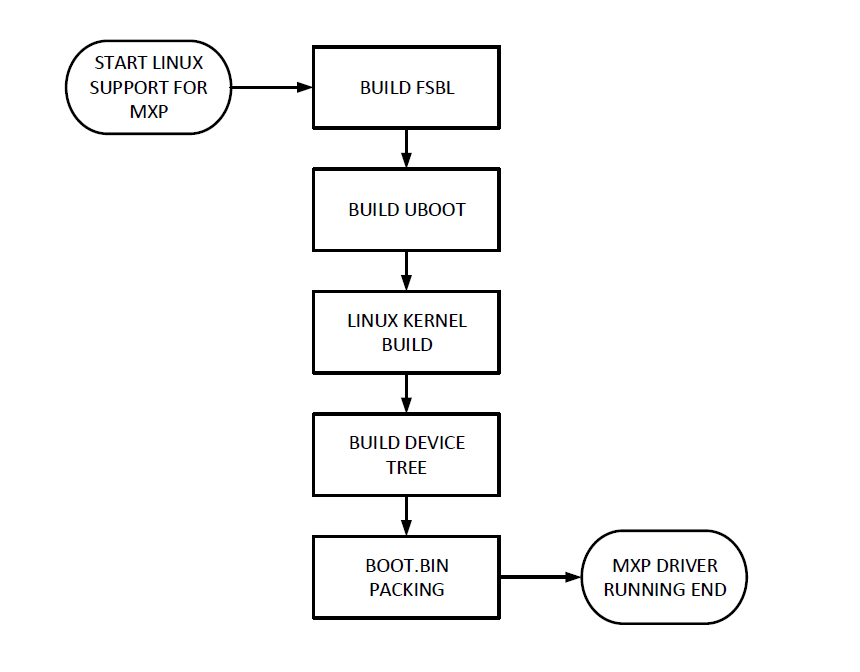
\includegraphics[width=.9\textwidth]{images/bootloader.png}
 
	\caption{Flowchart for Linux setup}
	\label{zed:boot}
\end{figure}



Inside the MXP repository, prebuilt bitstream (named system wrapper.bit to be instantiated on the FPGA) and hardware design file (named system.hdf) have been provided for 8 and 16 vector lanes configuration. We used the one with 16 vector lanes. Steps for setting up Linux on the ZedBoard for MXP are represented using the flowchart shown in figure~\ref{zed:boot} and have been explained in detail later in this chapter.

\section{Building First Stage Bootloader}


Inside the MXP repository, navigate to folder prebuilt\_zedboard\_arm\_viv\_v16 and type commands shown next. Once done rename executable.elf inside mxp\_fsbl to fsbl.elf.


\lstinputlisting[language=c,firstline=96, lastline=101, frame=none,numbers=left,basicstyle=\fontsize{11}{11}\selectfont\ttfamily, backgroundcolor=\color{gainsboro}]{codes.c}

\section{Building U-BOOT}

\begin{enumerate}
	\item Navigate to u-boot repository. We plan to use persistent filesystem rather than ramdisk. Below modifications are necessary in file include/configs/zynq common.h. Find sdboot entry and edit it. This is used to avoid loading ramdisk and make the filesystem persistent.
	
	\lstinputlisting[firstline=1, lastline=14, frame=none,numbers=left,basicstyle=\fontsize{11}{11}\selectfont\ttfamily, backgroundcolor=\color{gainsboro}]{CodeSnippet.txt}
	
	\item Then to compile u-boot give commands as shown below:
		\lstinputlisting[firstline=16, lastline=20, frame=none,numbers=left,basicstyle=\fontsize{11}{11}\selectfont\ttfamily, backgroundcolor=\color{gainsboro}]{CodeSnippet.txt}
		
\end{enumerate}

We renamed u-boot to u-boot.elf and while building Linux kernel we need mkimage utility, so add the tools/ folder to the \$PATH variable.

\section{Linux Kernel Build}

\begin{enumerate}
	\item Navigate to Linux repository and type the following commands.
	
	\lstinputlisting[firstline=22, lastline=23, frame=none,numbers=left,basicstyle=\fontsize{11}{11}\selectfont\ttfamily, backgroundcolor=\color{gainsboro}]{CodeSnippet.txt}
	
	This will generate a .config file.
	
	\item For building the kernel supporting the MXP we need to find out the necessary configuration parameters which needs to be tweaked. To do this, we do reverse engineering. If we look at example source codes provided in the bmark (benchmark) directory of MXP repo, we see the first function to be called in these sample examples is vbx\_test\_init(). For these source codes to run on Linux, this function calls VectorBlox MXP Initialize ("mxp0", "cma"). If we look at the definition of this function, it uses device files \/dev\/mxp0 and \/dev\/cma to do some memory mapping and other initializations. Since these device files are used, there must be corresponding device drivers for them in the Linux source. We surely find files named mxp.c and cma.c in the drivers/char/ directory which are responsible for creating these device files. We then look at the Makefile in drivers/char/ directory and find entries for these files as shown below:
	
	\lstinputlisting[firstline=25, lastline=26, frame=none,numbers=left,basicstyle=\fontsize{11}{11}\selectfont\ttfamily, backgroundcolor=\color{gainsboro}]{CodeSnippet.txt}
	
	Now we have the configuration parameters and hence we edit the .config file generated in step 1 and set these parameters as :
	
	\lstinputlisting[firstline=28, lastline=29, frame=none,numbers=left,basicstyle=\fontsize{11}{11}\selectfont\ttfamily, backgroundcolor=\color{gainsboro}]{CodeSnippet.txt}
	
	\item Compile the kernel and kernel modules:
	\lstinputlisting[firstline=31, lastline=32, frame=none,numbers=left,basicstyle=\fontsize{11}{11}\selectfont\ttfamily, backgroundcolor=\color{gainsboro}]{CodeSnippet.txt}
	
	This will generate compiled kernel uImage in arch/arm/boot/ directory.
	
	\item Insert the SD card with Xillybus setup into the computer where this kernel is compiled and give:
	
		\lstinputlisting[firstline=34, lastline=35, frame=none,numbers=left,basicstyle=\fontsize{11}{11}\selectfont\ttfamily, backgroundcolor=\color{gainsboro}]{CodeSnippet.txt}
		
	This will copy all the kernel modules built in step 4 into the path: IN-
	STALL MOD PATH/lib/modules/\{kernel image name\}/
	
\end{enumerate}

\section{Building Device Tree}

\begin{enumerate}
	\item Inside Linux repo, compile device tree source (dts) to generate device tree blob (dtb).

	\lstinputlisting[firstline=37, lastline=40, frame=none,numbers=left,basicstyle=\fontsize{11}{11}\selectfont\ttfamily, backgroundcolor=\color{gainsboro}]{CodeSnippet.txt}	
	
	To avoid using ramdisk, we replace the contents of bootargs under the chosen node in mxp\_linux.dts as shown:
	
		\lstinputlisting[firstline=42, lastline=46, frame=none,numbers=left,basicstyle=\fontsize{10}{11}\selectfont\ttfamily, backgroundcolor=\color{gainsboro}]{CodeSnippet.txt}
		
	\item Copy folders from drivers/ directory inside MXP repo to the Device tree repo. Navigate to folder prebuilt zedboard\_arm\_viv\_v16 in MXP repo, and enter following commands:
	
			\lstinputlisting[firstline=48, lastline=55, frame=none,numbers=left,basicstyle=\fontsize{11}{11}\selectfont\ttfamily, backgroundcolor=\color{gainsboro}]{CodeSnippet.txt}
			
			\begin{figure}
				\centering
				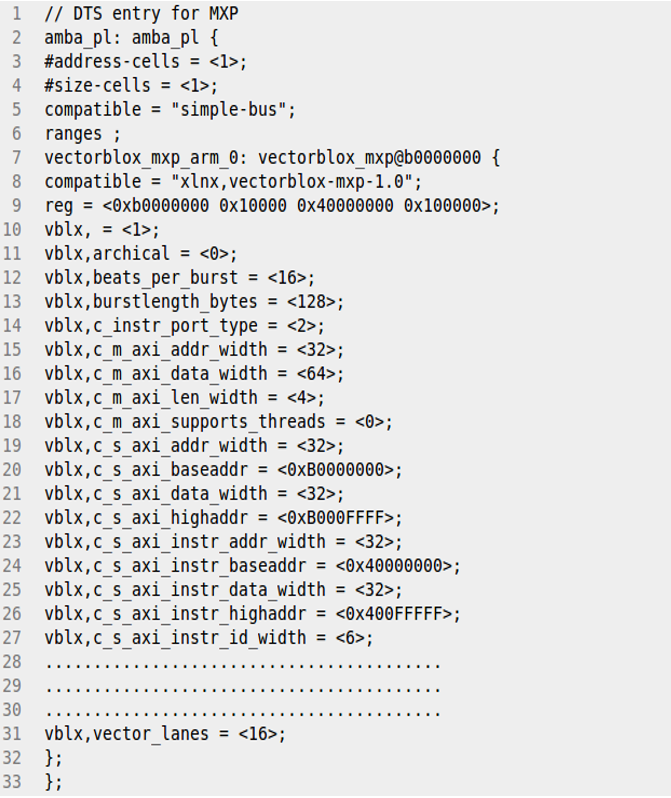
\includegraphics[width=1\textwidth]{images/c4.png}
				\caption{DTS Entry for MXP}
				\label{dts:blk}
			\end{figure}
			
			After this, we see some dts\/dtsi files created inside mxp\_dts folder. We already have the device tree entries corresponding to various peripherals in mxp\_linux.dts file created in step 1. Hence, we are only interested in pl.dtsi files which will contain the device tree node for the MXP soft processor instantiated on programmable logic. Contents in pl.dtsi is as shown in Figure~\ref{dts:blk}.
		
		Given the way in which the device driver file mxp.c parses this device tree
		node, we need to change contents of this file for the correct setup Specifically we need to change compatible string to
	
	\lstinputlisting[firstline=57, lastline=57, frame=none,numbers=left,basicstyle=\fontsize{11}{11}\selectfont\ttfamily, backgroundcolor=\color{gainsboro}]{CodeSnippet.txt}	
	
	Also, the register entry should contain instruction address first. So, node name and reg entry should be changed to
	
		\lstinputlisting[firstline=59, lastline=60, frame=none,numbers=left,basicstyle=\fontsize{11}{11}\selectfont\ttfamily, backgroundcolor=\color{gainsboro}]{CodeSnippet.txt}	
		
		Copy the edited amba\_pl node to the end of mxp\_linux.dts.
		
		\item Finally the device tree is compiled.
	
\lstinputlisting[firstline=62, lastline=62, frame=none,numbers=left,basicstyle=\fontsize{11}{11}\selectfont\ttfamily, backgroundcolor=\color{gainsboro}]{CodeSnippet.txt}			
		
			
\end{enumerate}
	
\section{Packing into BOOT.bin}

Create a file with name, say bootimage.bif. Paste following contents into it

\lstinputlisting[firstline=64, lastline=72, frame=none,numbers=left,basicstyle=\fontsize{11}{11}\selectfont\ttfamily, backgroundcolor=\color{gainsboro}]{CodeSnippet.txt}	

Save the file and generate boot.bin using the command below:

\lstinputlisting[firstline=74, lastline=74, frame=none,numbers=left,basicstyle=\fontsize{11}{11}\selectfont\ttfamily, backgroundcolor=\color{gainsboro}]{CodeSnippet.txt}

Copy files boot.bin, devicetree.dtb and uImage into the FAT partition of sdcard. Plug-in the sdcard and boot ZedBoard. While the kernel is getting loaded we should some message like this

\lstinputlisting[firstline=76, lastline=81, frame=none,numbers=left,basicstyle=\fontsize{11}{11}\selectfont\ttfamily, backgroundcolor=\color{gainsboro}]{CodeSnippet.txt}

This means mxp driver is successfully loaded.

\section{Configuration Parameters of MXP}
We successfully loaded the MXP drivers. The configuration parameters for the MXP setup includes some important parameters named as below:
\begin{enumerate}

	\item vector\_lanes.

	\item core\_freq.

	\item scratchpad\_size.

	\item dma data width in bytes.
 
\end{enumerate}

\lstinputlisting[firstline=83, lastline=87, frame=none,numbers=left,basicstyle=\fontsize{11}{11}\selectfont\ttfamily, backgroundcolor=\color{gainsboro}]{CodeSnippet.txt}


\section{Code for Configuration in Detail}

The configuration details can be found in the below link:

Github Link : \url{https://github.com/AdhikariSaurabh/mxpbenchmarks}

